\documentclass{bioinfo}
\copyrightyear{2015}
\pubyear{2015}
\usepackage[english]{babel}
\usepackage{amssymb,amsfonts,amsmath}
\usepackage{hyperref}
\usepackage{graphicx}
\usepackage{amsmath}
\usepackage{natbib}

\newcommand{\EQ}[1]{Eq.~(\ref{eq:#1})}
\newcommand{\EQS}[2]{Eqs.~(\ref{eq:#1}) and (\ref{eq:#2})}
\newcommand{\FIG}[1]{Fig.~\ref{fig:#1}}
\newcommand{\TAB}[1]{Tab.~\ref{tab:#1}}
\newcommand{\REF}[1]{ref.~\citep{#1}}



%%%%%%%%%%%%%%%%%%%%%%%%%%%%%%%%%%%%%%%%%%%%%%%%%%%%%%%%%%%%%%%%%%%%%%%%%%%%%%
\begin{document}
%%%%%%%%%%%%%%%%%%%%%%%%%%%%%%%%%%%%%%%%%%%%%%%%%%%%%%%%%%%%%%%%%%%%%%%%%%%%%%
\title[Tracking of seasonal influenza H3N2 virus evolution]{nextflu: Real-time tracking of seasonal influenza H3N2 virus evolution in humans}
\author{Richard~A.~Neher$^{1}$ and Trevor Bedford$^{2}$}
\address{$^{1}$Max Planck Institute for Developmental Biology, 72076 T\"ubingen, Germany, and $^{2}$Vaccine and Infectious Disease Division, Fred Hutchinson Cancer Research Center, Seattle, WA 98109, USA}
\history{Received on XXXXX; revised on XXXXX; accepted on XXXXX}

\editor{Associate Editor: XXXXXXX}

%\date{\today}
\maketitle
\bibliographystyle{plain}


%%%%%%%%%%%%%%%%%%%%%%%%%%%%%%%%%%%%%%%%%%%%%%%%%%%%%%%%%%%%%%%%%%%%%%%%%%%%%%
\begin{abstract} \section{Summary:} Seasonal influenza viruses evolve rapidly and change their antigenic properties.
This allows the virus population to evade immunity in their human hosts and reinfect previously infected individuals.
Similarly, vaccines against seasonal influenza need to be updated frequently to protect against an evolving virus population.
We have thus developed a processing pipeline and web-browser based visualization that allows convenient exploration and analysis of the most recent influenza virus sequence data.
This web-application displays a phylogenetic tree that can be decorated with additional information such the viral genotype at specific sites, sampling location, and sequence or tree based statistics that have been shown to predictive of future virus dynamics.
Additionally, mutation frequency trajectories are calculated and displayed.

\section{Availability and implementation:} Python and Javascript source code is freely available from \url{https://github.com/blab/nextflu}, while the web-application is live at \url{http://nextflu.org}.

\section{Contact:} tbedford@fredhutch.org

\end{abstract}
%%%%%%%%%%%%%%%%%%%%%%%%%%%%%%%%%%%%%%%%%%%%%%%%%%%%%%%%%%%%%%%%%%%%%%%%%%%%%%

%%%%%%%%%%%%%%%%%%%%%%%%%%%%%%%%%%%%%%%%%%%%%%%%%%%%%%%%%%%%%%%%%%%%%%%%%%%%%%
\section*{Introduction}

\begin{itemize}
	\item Motivation
	\item data sources
	\item pipe line and design
	\item frequency estimation details
	\item genotype and trait coloring
	\item generalizability
\end{itemize}

nextflu consists of a processing pipeline writtin in python and a javascript based visualization called auspice.
As input, augur requires a fasta file of sequences of the HA segment with fasta labels containing relevant information such as the strain name, the sampling date and passage history.
In a first step, viruses without complete date  or geographic information and viruses passaged in eggs are removed.
In addition, local outbreaks are filtered by keeping only one instance of identical sequences sampled at the same location on the same day.
Following filtering, the viruses are subsampled to achieve an appoximately even temporal and global distribution (typically 50 viruses per month).
For our standard display period of 3 years, this typically results in \~1800 viruses, which we align us \texttt{mafft} \citep{mafft}.

Once aligned, the set of virus sequences is further cleaned by removing insertions relative to the outgroup and by removing sequences that are either much closer or further from the outgroup then expected given their date of sampling (filtering viruses that don't follow an approximate molecular clock).
REASSORTANTS.

From the filtered and cleaned alignment, augur builds a phylogenetic tree using \texttt{fasttree} \citep{Price:2009p47657} which is further refined by one hour of RAxML optimization \citep{RAxml}.
Next, the state of every internal node of the tree is inferred using marginal maximum likelihood method and missing sequence is filled with the nearest ancestral sequence.
Internal branches without mutations are collapsed into polytomies.
The final tree is decorated with the attributes to be displayed in the browser, see below.  

\begin{figure}[t!]
	\begin{center}
	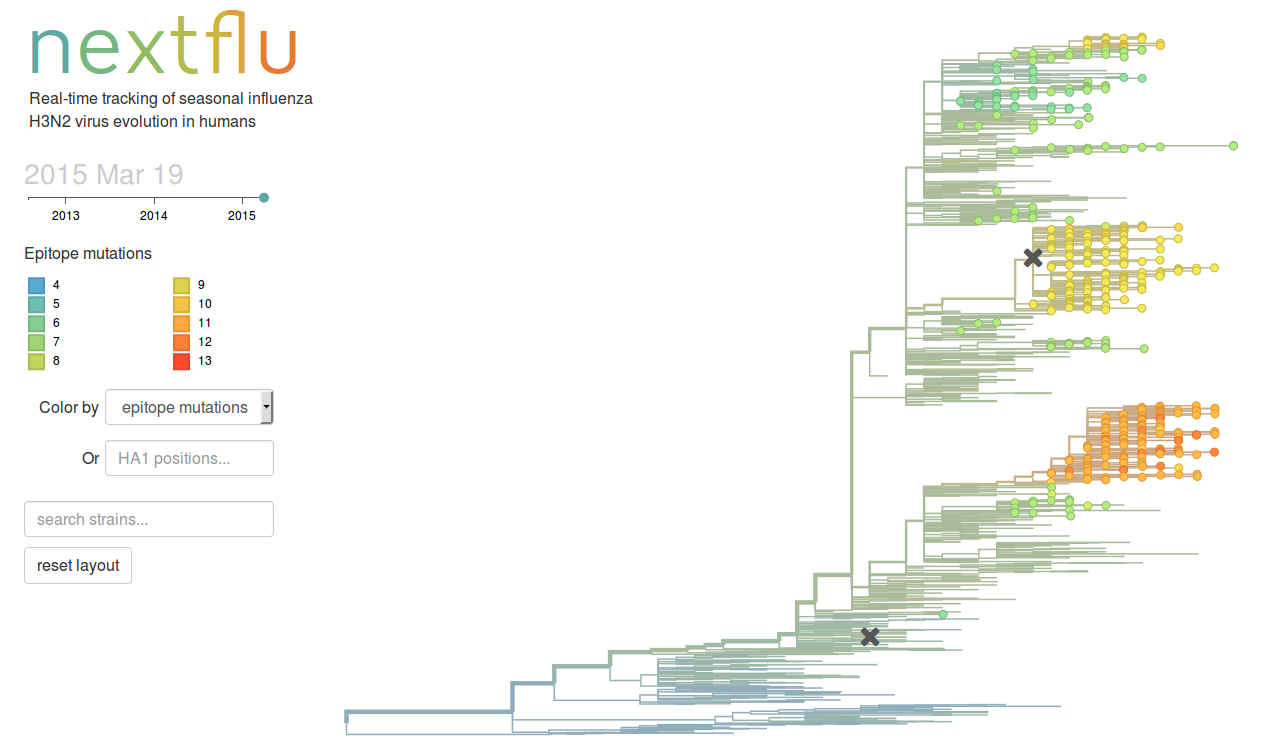
\includegraphics[width=0.99\columnwidth]{figures/tree_screenshot}
\caption[]{The \texttt{nextflu} website with the user interface on the left and
the tree on the right.}
\label{fig:tree}
\end{center}
\end{figure}

In addition to the phylogenetic tree, augur estimates the frequency trajectories of mutations, genotypes and clades in the tree. 
Frequency trajectories are represented as a linear interpolation $x(t)$ of values $x_i$ at time points  $t_i$ spaced one month apart. 
The pivot frequencies corresponding to a feature $\phi$ (e.g. mutation) are estimated by minimizing
\begin{equation}
\label{eq:freq}
	\begin{split}
	-\log LH(\{x_i\} | \phi)  =& \sum_v I(v,\phi)\log(x(t_v)) + (1-I(v,\phi))\log(1-x(t_v)) \\
			&+\sum_i \frac{(\Delta x_i - \epsilon\Delta x_{i-1})^2}{2\gamma \delta t_i}
\end{split}
\end{equation}
where $I(v,\phi)=1$ if virus $v$ carries attribute $\phi$ and $I(v,\phi)=0$ otherwise.
$\Delta x_i = x_i-x_{i-1}$, $\Delta t_i = t_i-t_{i-1}$, $\gamma$ parameterizes the smoothing imposed on the frequency estimate (related to the frequency changes by genetic drift) and $\epsilon$ parameterizes our expectation of frequency changes in interval $i$ based on the observed change in interval $i-1$.
$\epsilon=0$ implies that frequency changes are uncorrelated from one interval to the next, while $\epsilon=1$ implies that
the most likely $\Delta x_i$ is $\Delta x_{i-1}$.
We typically use $\epsilon = 0.7$.
\EQ{freq} is minimized using SciPy's implementation of a downhill simplex algorithm \citep{Oliphant:2007p25672}.
To speed up convergence, minization is first done using a coarse grid of pivot points which is
subsequently refined to 12 pivots per year.
PUT IN DETAILS ON HOW WE ESTIMATE FREQUENCIES ON THE TREE?

The tree decorated with attributes and clade frequencies is written to file in a nested json format for display in the browser by auspice.
In addition to the tree, json files containing the sequences, frequencies of mutations and genotypes, as well as meta information are exported.

The tree is visualized by auspice using d3 \citep{d3}.
The user can explore the data interactively by selecting viruses from different dates (moving the date slider, top right corner in \FIG{tree}) or by coloring the tree by the following attributes:
\begin{itemize}
	\item epitope mutations: each tip is colored by the number of aminoacid mutations at \~50 positions relative to the root of the tree.
These positions are known to be frequent targets of antibodies \citep{shih_simultaneous_2007} and have been suggested to be predictive of future success \citep{luksza_predictive_2014}.
	\item non-epitope mutations: color by the number of mutations outside the above mentioned epitope sites.
	Mutations outside epitopes tend to be damaging and anti-correlated with clade expansion \citep{luksza_predictive_2014}.
    \item receptor binding mutations: color by the number of mutations at 7 positions close to the receptor binding site that have been shown to be responsible for major antigenic positions in the past decades \citep{koel_substitutions_2013}.
    \item local branching index is the exponentially weighted tree length surrounding a node, which is associated with rapid branching and expansion of clades \citep{neher_predicting_2014}.
It is recalculated everytime the date slider is moved and based only on the highlighted viruses.
    \item geographic location
    \item HA1 genotype: entering amino acid positions (separated by a comma) in the text field will color every node according to the genotype at these positions.
\end{itemize}

The frequency plot below the tree (see \FIG{freq}) displays the frequency trajectory of clades in the tree whenever the mouse hovers above the branch defining the clade. 
Furthermore, trajectories of individual mutations, combinations of two mutations, and predifined clades such as 3c3.a can be plotted by entering them in text field.

\begin{figure}[bhtp]
	\begin{center}
	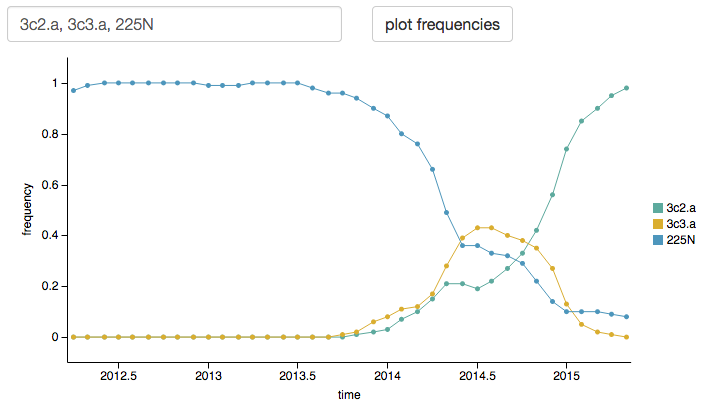
\includegraphics[width=0.99\columnwidth]{figures/frequencies}
\caption[]{The frequency diagram on \url{nextflu.org} allows geography specific
		plotting of frequencies of individual mutations, pairs of mutations, 
		predefined genotypes, as well as clades in the tree. }
\label{fig:freq}
\end{center}
\end{figure}

\section{Conclusion}
We built nextflu.org to facilitate the analysis and exploration of seasonal influenza sequence data collected by laboratories around to world.
By using the most recent data and integrating phylogenies with frequency trajectories and sequence or tree based predictors of successful clades, we hope that nextflu can inform the choice of strains used in seasonal influenza vaccines. 

nextflu was designed to be readily adapted to other rapidly evolving viruses. To that end, the generic classes used for processing the sequence data to include features specific to the virus in question. 

\paragraph{Funding\textcolon}This work is supported by the ERC though Stg-260686.

%%%%%%%%%%%%%%%%%%%%%%%%%%%%%%%%%%%%%%%%%%%%%%%%%%%%%%%%%%%%%%%%%%%%%%%%%%%%%%
\bibliography{nextflu}
%%%%%%%%%%%%%%%%%%%%%%%%%%%%%%%%%%%%%%%%%%%%%%%%%%%%%%%%%%%%%%%%%%%%%%%%%%%%%%
\end{document}
%%%%%%%%%%%%%%%%%%%%%%%%%%%%%%%%%%%%%%%%%%%%%%%%%%%%%%%%%%%%%%%%%%%%%%%%%%%%%%
